\documentclass[crop,tikz]{standalone}

\usepackage{amsmath}
\tikzset{>=latex}
\usetikzlibrary{patterns,decorations.pathmorphing}

\begin{document}
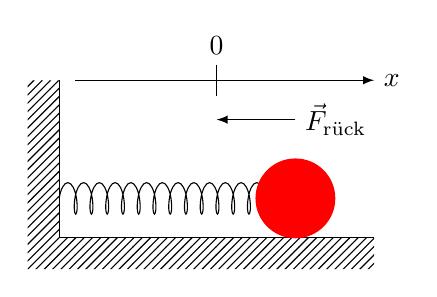
\begin{tikzpicture}[scale=2]
  \draw[->] (-0.9,1) -- (1,1) node[right] {$x$};
  \draw (0,0.9) -- (0,1.1) node[above] {$0$};
  \draw (-1,1) -- (-1,0) -- (1,0);
  \pattern[pattern=north east lines,pattern color=black] (-1.2,1)--++(0.2,0)--++(0,-1)
  --++(2,0)--++(0,-0.2)--++(-2,0)--++(-0.2,0)--cycle;
  \draw[decoration={aspect=0.3, segment length=2mm, amplitude=2mm,coil},decorate] (-1,0.25) -- (0.5,0.25);
  \draw[red,fill] (0.5,0.25) circle (0.25);
  \draw[->] (0.5,0.75) node[right]{$\vec{F}_\text{rück}$} -- (0,0.75);
\end{tikzpicture}
\end{document}
